% notes/todo

TODO: Something about the dispatchers and about what happen when things go right (near-miss)


Traditionally, safety systems are modelled as complex linear system, rather than non-linear.

\chapter{Terminology}
In general it is not recommended to say that a specific event (X) causes another (Y). This implies that X is a precondition to Y, and by eliminating X\footnote{Methods for accident investigation}

Safety: freedom from unacceptable risk

TODO: explain risk matrix

\section{Near miss}
%A near miss is an unplanned event that did not result in injury, illness, or damage – but had the potential to do so. Only a fortunate break in the chain of events prevented an injury, fatality or damage; in other words, a miss that was nonetheless very near. Although the label of 'human error' is commonly applied to an initiating event, a faulty process or system invariably permits or compounds the harm, and should be the focus of improvement. Other familiar terms for these events is a "close call", or in the case of moving objects, "near collision".

\section{Resonance}

Resonance is a phenomenon in physics making a system oscillate at a higher amplitude when a force is applied.

\section{ATC}
\label{sec:atc}
ATC, or Automatic Train Control is a mechanism that allows automatic interlocking of railway blocks.

Barrier in safety engineering

general safety en resilience engineering terminology

\section{Railway}

%Single-track and dual track operation

\subsection{Block}
A block is a distance of railway that, at any point in time can only be occupied by one train. There are two types of blocks; fixed and moving.

Traditionally, railways are divided into a number of fixed blocks with entry and exit signals. These signals will represent train movement along the block based on a predefined policy. The policy is again determined from a number of parameters:


\begin{itemize}
  \item The permitted maximum speed on the line
  \item The maximum speed and braking characteristics of the different trains occupying the track
  \item Geological conditions, such as gradients, as these could lead to increase in breaking time.
  \item Line-of-sight. Being that the signal is optical, the train driver must be able to see it before acting on it.
  \item The reaction time of the driver
\end{itemize}
Whereas the maximum speed and geological conditions can be modelled linear - the response time of the driver cannot. And on a line without ATC (see section \ref{sec:atc}) failure to observe a non-go signal will effectively cancel out all other factors in the model.


%Ideally, block interlocking policy should be set to match something like

%TODO - change this formula

%$T_{blocking} = 2*WCGF*(WCBT + WCRT)$

%Where

%\begin{itemize}
%  \item $T_{blocking}$ is the amount of time a 
%  \item $WCGF$ is the worst case gradient factor
%  \item $WCBT$ is the worst case braking time
%  \item $WCRT$ is the worst case response time of the driver
%\end{itemize}
Fixed blocks wastes a lot of capacity, as most blocks go largely unused for most of their distance, plus there is a lot of overhead on stopping times.

Moving block address this issue. Instead of having the line divided into a number of fixed blocks, a "safe distance" is defined dynamically based on the current speed and location of the train.
This greatly increases the requirement for the technological infrastructure, and the dependability of it.

Safety has always been a high priority in railway engineering and deployment, and it has thus been a largely contributing industry to safety critical research.

Railway safety is largely dependant on supervision systems, and dispatchers.

\subsection{Timetable}
The primary barrier to provide safety in railway operation is the timetable. It specifies which trains are supposed at a certain location at a certain point in time.

\subsection{Dispatcher}
A train dispatcher can be considered the safety net for when the static timetable needs to altered mid-deployment.
Dispatchers act on



\cite{belmonte2008dispatcher}


\section{Safety systems}

\section{Classic model on safety}
%http://en.wikipedia.org/wiki/Swiss_cheese_model
Barriers are depicted as layers of swiss cheese with holes in them. 


There has been a paradigm shift in the view on accidents in the later years. Now, accidents are not considered a linear succession events, but rather a complex combination of events.


%**Stolen
%Cognitive Reliability and Error Analysis (CREAM) [5]. CREAM allows to highlight the dependence of human performance on the context and provides an useful cognitive model for both retrospective and prospective acci-dent analysis. The specificity of CREAM is that human errors are shaped more bythe context than by a stochastic process.
%/stolen

\section{Resilience Engineering}
\label{sec:resilience_engineering}
Resilience engineering can be considered the complimentary to safety engineering; where as safety engineering seeks to build a better and safer system, resilience engineering embraces the fact that errors arise within a system - and tries to limit the impact of these.

Whereas traditional risk management rely largely on lessons learned, and empric data to provide probabilities; resilience engineering provocatively seeks to create safety though flexibility. Meaning that when a sub-system breaks down it does not necessarily mean the breakdown of the entire system.

Dynamic reconfiguration is a good example on resilience engineering.
%TODO example

Basically it cuts down to the the following question: "If this component breaks down - how will the rest of the system react, and how can I limit the impact."

%**Stolen
%Resilience Engineering looks for ways to enhance the aility of organisations to create processes that are robust yet flexible, to monitor and revise risk models, and to use resources proactively in the face of disruptions or ongoing production and economic pressures. 
%In Resilience Engineering failures do not stand for a breakdown or malfunctioning of normal system functions, but rather represent the converse of the adaptations necessary to cope with the real world complexity. Individuals and organisations must always adjust their performance to the current conditions; and because resources and time are finite it is inevitable that such adjustments are approximate. Success has been ascribed to the ability of groups, individuals, and organisations to anticipate the changing shape of risk before damage occurs; failure is simply the temporary or permanent absence of that.
%/Stolen


\section{Human factors}
The variability of is system is becoming more and more dependent on individual and/or collective performance of humans.

Historically, this has not always been so.
%TODO

\subsubsection{Circadian rhythm}
The circadian rhythm is a the natural daily rhythm that is found in, humans, plants, other mammals alike. It has tremendous impact on the performance of an individual and is thus non-negligible when discussing human factors in a system.

Circadian rhythm has a large impact on, for example aeroplane pilots flying across time zones, and thus loses their natural sense of daylight. This leads to fatigue, decreased responsiveness and performance (\cite{mallis2010aircrew}).
%TODO - Add licenseing
\begin{figure}[h]
 \centering
   \includegraphics[width=360pt]{figures/biological_clock_human.pdf}
 \caption{Human biological clock \\(Licence: GFDL)}
 \label{fig:human_biological_clock}
\end{figure}


\subsection{•}
%**Stolen
% The understanding of the human role in accidents has gone through three stages. In the classical view, humans were seen as error prone or as fallible machines. The purpose of an accident investigation was therefore often to find the "human error" that either was the primary (or even "root") cause or the initiating event.
%When it became clear, in the 1990s, that the "human error" view was not tenable, explanations changed to look for how performance shaping factors or performance conditions could make people fail, in the sense of "forcing" errors. This did not remove the concept of a "human error", but saw these as a product of the working conditions and work pressures, rather than as a result of built-in human error tendencies.
%Although this development enabled people to understand accidents of a more complex nature for a while, it still fell short in a number of situations. This led to the recognition, strongly supported by resilience engineering, that failures and successes have the same source, and that they metaphorically speaking are two sides of the same coin.
%The functional resonance model (Hollnagel, 2004) describes system failure as a resonance of the normal variability of functions. To arrive at a description of functional variability and resonance, and to determine recommendations for damping unwanted variability, a FRAM analysis consists of four steps:

%Identify and describe essential system functions, and characterise each function by six basic parameters.
%Characterise the (context dependent) potential variability through common performance conditions.
%Define the functional resonance based on possible dependencies / couplings among functions and the potential for functional variability.
%Identify barriers for variability (damping factors) and specify required performance monitoring.
%/Stolen
\subsection{Functional Resonance Analytic Model}
%The functional resonance accident model (FRAM; Hollnagel, 2004) describes system failure in terms of the resonance of normal performance variability. This provides a convenient way of representing the non-linear propagation of events and also makes it possible to account for adverse outcomes in cases where there were no manifest malfunctions or failures. The principle of FRAM is to characterise individual system functions independently of how they may be connected in a specific situation. The characterisation of each function ­ or node ­ is done in terms of six aspects and the values of these aspects determine how nodes may be coupled under given conditions. To produce a description of functional variability and potential resonance, and to determine recommendations for damping unwanted variability, a FRAM analysis consists of four steps:


FRAM is designed for systems which both include human and organizational factors.

(Difference between method and model.)


\section{FRAM tools}
A special-purpose piece of computer software exists to visualize the FRAM models and conveniently describe the functions and couplings using textual input and graphical representation.

\begin{figure}[h]
 \centering
   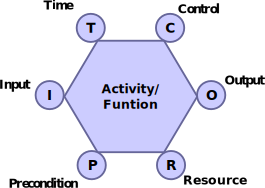
\includegraphics[width=200pt]{figures/FRAM_node.pdf}
 \caption{FRAM node}
 \label{fig:fram_node}
\end{figure}


Each node consists of a number of edge connection points  which model

\begin{itemize}
  %Time available: This can be a constraint but can also be considered as a special kind of resource
  \item Time: Time constraints. When a function is dependant on a time input, this connects to and output port of another node.

%Precondition: System conditions that must be fulfilled before a function can be carried out.
  \item Precondition: A connected function must supply output to this input before the function can start.

% Control: That which supervises or adjusts a function. Can be plans, procedures, guidelines or other functions.
  \item Control: Implies "controlled by", and specifies input from supervising function
  
%Input: That which is used or transformed to produce the output. Constitutes Input the link to previous functions.
  \item Input: That which is used or transformed to produce the output. Constitutes the link to previous functions.

%Output: That which is produced by function. Constitute Output links to subsequent functions.
  \item Output: The product of this function
%Resource: That which is needed or consumed by function to process input (e.g.,matter, energy, hardware, software, manpower).
  \item Resource: Resources consumed by this function (e.g.,matter, energy, hardware, software, manpower)
\end{itemize} 


FRAM analysis basically consists of four steps:

\subsubsection*{Step 1}
%Step 1: Identify essential system functions, and characterise each function by six basic aspects or parameters. The six aspects are input (I, that which the function uses or transforms), output (O, that which the function produces), preconditions (P, conditions that must be fulfilled to perform a function), resources (R, that which the function needs or consumes), time (T, that which affects time availability), and control (C, that which supervises or adjusts the function). Nodes and their aspects may be described in a table and can subsequently visualized in a hexagonal representation (cf. Figure 2 and 4 below).
The objective of the first step is to identify essential system functions, and characterise each of them by the six basic aspects specified in figure \ref{fig:fram_node}. This can be done in a table, and converted to hexagonal objects later on.
%TODO
\subsubsection*{Step 2}
%Step 2: Characterize the context dependent variability of each node. For an accident analysis, the variability is known from the investigation data. In this case the analysis focuses on comparing the observed and the normal performance. For risk assessment, the variability may be derived from a characterisation of the common performance conditions (CPCs), of which there currently are eleven. These CPCs address the combined human, technological, and organizational aspects of each function. After identifying the CPCs, the variability must be determined in a qualitative way in terms of stability, predictability, sufficiency, and boundaries of performance. 
The next step is to characterize the context dependent variability of each node from a list of common performance conditions - or CPCs. 
%TODO list the eleven CPCs
\begin{itemize}
  \item CPC 1
  \item CPC 2  
\end{itemize}

After identifying the CPCs, the variability must be determined in a qualitative way in terms of stability, predictability, sufficiency, and boundaries of performance. 

When applied on an accident analysis, the analysis focuses on comparing the observed and the normal performance.

%**Stolen

\subsubsection*{Step 3}
%Step 3: Defining the functional resonance based on possible dependencies/couplings among functions and the potential for functional variability. The output of the functional description of step 1 is a characterisation of functions and their aspects. The aspects provides the basis for identifying how functions may be coupled. For example, the output of one function may be an input to another function, or produce a resource, fulfil a pre-condition, or enforce a control or time constraint. When the couplings between functions are found, this is combined with the characterization of performance variability from Step 2. In this way the analysis will show how the variability of one function may have an impact on others. This analysis thus determines how resonance, and ultimately adverse outcomes, can result from variability across functions in the system. For example, if the output of a function is unpredictably variable, another function that depends on this output as a resource may be performed unpredictably. Many such occurrences and propagations of variability may have an effect like resonance.
The third step will link the functions and define the functional resonance


%Step 4: Identify barriers for variability (damping factors) and specify required performance monitoring. Barriers are hindrances that may either prevent an unwanted event from taking place, or protect against the consequences (Hollnagel, 2004). Barriers can be described in terms of barrier systems (the organizational and/or physical structure of the barrier) and barrier functions (the manner by which the barrier achieves its purpose). In FRAM, four categories of barrier systems are identified (each with their potential barrier functions, see Hollnagel, 2004). In addition to recommendations for barriers, FRAM can also be used to specify recommendations for the monitoring of performance and variability, as a way to detect and manage undesired variability. Performance indicators may thus be developed for every function and every link between functions.
\subsection*{Sted 4}
The final step will be be the remedial one, where identification of variability barriers - or damping factors - will take place.


\subsection{Barrier}
Barriers are hindrances that may either prevent an unwanted event from taking place, or protect against the consequences (Hollnagel, 2004)

\subsection{Fram Visualizer}


\begin{figure}
 \centering
   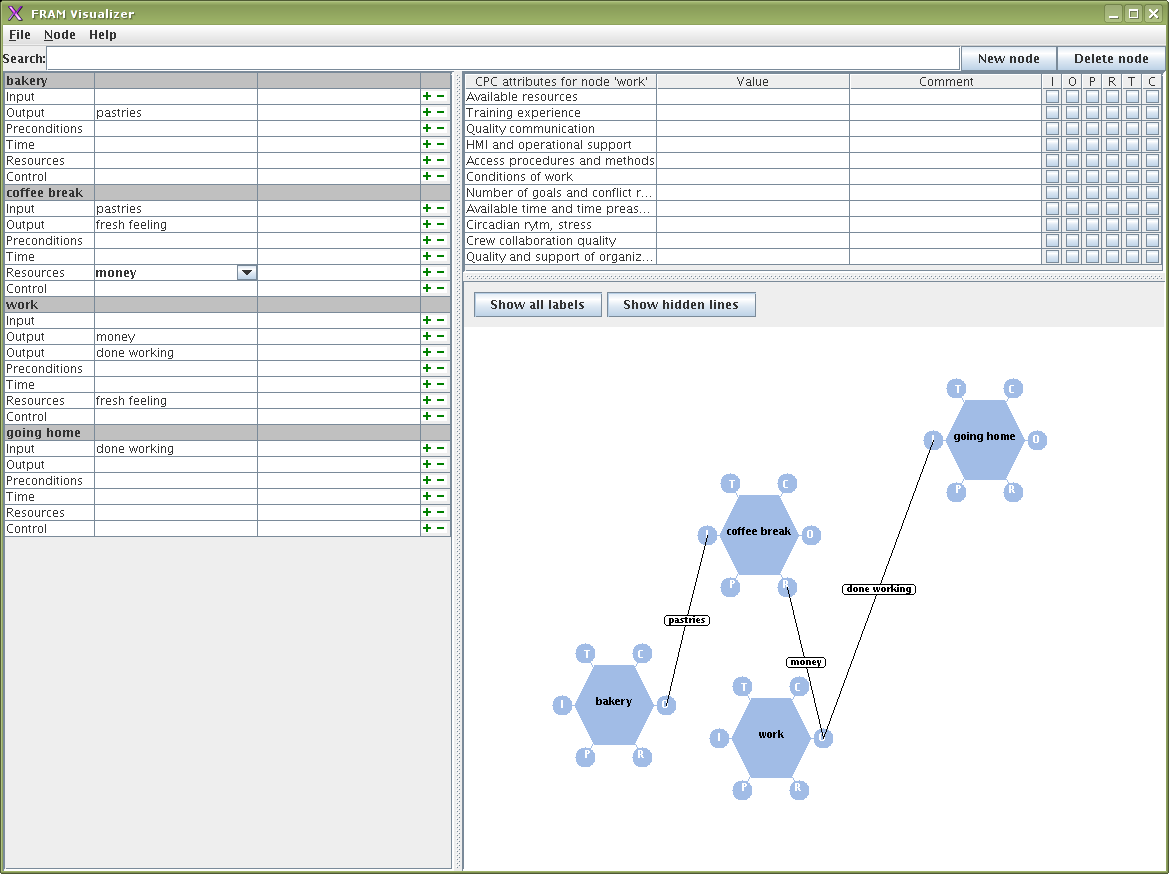
\includegraphics[width=320pt]{figures/framvisualizer1.png}
 \caption{FRAM Visualizer interface}
 \label{fig:fram_visualizer_interface}
\end{figure}

\section{Retrospective FRAM}
Although FRAM is intended to be used as a design-phase tool to enhance the recilience of a system (or sub-system), its modeling characteristics enables it to be applied retrospective on an accident or near-miss event.

%**Stolen
%How to use FRAM for event analysis (retrospective)
%An analysis using FRAM comprises the following five steps:
%Define the purpose of modelling and describe the situation being analysed. Either an event that has occurred (incident/accident) or a possible future scenario (risk).
%Identify the essential functions that make up the event ('foreground' functions – when things go right); characterise each by six basic aspects (Input, Output, Pre-conditions, Resources, Time, and Control). 
%Characterise the actual / potential variability of 'foreground' functions and 'background' functions (context). Consider both normal and worst case variability.
%Define functional resonance based on potential  / actual dependencies (couplings) among functions.
%Propose ways to monitor and dampen performance variability (indicators, barriers, design / modification, etc.)
%/Stolen



